% ============================================================
%  Chương III – Cấu trúc hạ tầng khóa công khai PKI
%  ~1000 từ · 3 trang
% ============================================================
\chapter{Cấu trúc hạ tầng khóa công khai PKI}
\label{chap:pki-arch}

% Ý chính: PKI không chỉ là kỹ thuật mà là hệ thống tổ hợp
% con người + quy trình + phần mềm + phần cứng + chính sách.
Hạ tầng khóa công khai (Public Key Infrastructure - PKI) thường bị nhầm tưởng chỉ là một tập hợp các thuật toán mã hóa và phần mềm. Tuy nhiên, trên thực tế, PKI là một hệ thống toàn diện, là sự tổ hợp chặt chẽ giữa con người, quy trình, phần mềm, phần cứng và các chính sách an toàn thông tin. Mục tiêu cốt lõi của hệ thống này là tạo ra, quản lý, phân phối, sử dụng, lưu trữ và thu hồi các chứng chỉ số một cách an toàn, từ đó thiết lập và duy trì nền tảng tin cậy cho các giao dịch điện tử trên môi trường mạng không an toàn.


% ----------------------------------------------------------
\section{Các mô hình phân phối khóa công khai}
\label{sec:3.1}
% Ý chính: 4 layer tiến hóa — host-based trust → centralized KDC → Web of Trust → hierarchical PKI
% Mỗi layer giải quyết một vấn đề của layer trước nhưng lại tạo ra vấn đề mới
Sự phát triển của các cơ chế phân phối khóa công khai trải qua nhiều giai đoạn tiến hóa, từ các phương pháp thủ công, đơn giản như Host-based Trust, phân tán như Web of Trust, cho đến các mô hình có tính hệ thống cao như Hierarchical PKI. Mỗi mô hình ra đời nhằm giải quyết những hạn chế của mô hình trước đó, nhưng đồng thời cũng phải đối mặt với những thách thức mới.

\subsection{Bài toán phân phối khóa công khai}
% Ý chính: public key cần được công bố rộng rãi nhưng vẫn phải đảm bảo tính bảo mật
% Bốn mục tiêu: xác thực, bảo mật, toàn vẹn, không chối cãi
Trong hệ mật mã bất đối xứng, khóa công khai (Public Key) được thiết kế để công bố rộng rãi cho bất kỳ ai muốn giao tiếp an toàn với chủ sở hữu của nó. Tuy nhiên, bài toán đặt ra là làm thế nào để phân phối khóa công khai này rộng rãi mà vẫn đảm bảo tính an toàn. Quá trình phân phối này cần hướng tới việc hỗ trợ bốn mục tiêu an toàn thông tin cơ bản: tính xác thực (Authentication), tính bảo mật (Confidentiality), tính toàn vẹn (Integrity) và tính chống chối bỏ (Non-repudiation).

\subsection{Public Announcement}
% Ý chính: public key được công bố rộng rãi, ai cũng có thể truy cập
% Ví dụ: DNSSEC public key được lưu trong DNS, có thể truy vấn bằng dig
% Vấn đề authentication: làm sao biết public key đó thực sự thuộc về entity nào?
Đây là phương pháp cơ bản nhất, trong đó khóa công khai được chia sẻ công khai trên một nền tảng dễ tiếp cận. Một ví dụ tiêu biểu là DNSSEC, nơi khóa công khai được lưu trữ trực tiếp trong các bản ghi DNS và bất kỳ ai cũng có thể truy vấn thông qua các công cụ như \texttt{dig}. Tuy nhiên, điểm yếu lớn nhất của phương pháp này nằm ở khả năng xác thực (Authentication), vì không có cơ chế đáng tin cậy nào để kiểm chứng xem khóa đó có thực sự thuộc về thực thể mà nó tự nhận hay không, dẫn đến tấn công Man-in-the-Middle.

\subsection{Host-based Trust}
% Ý chính: SSH known\_hosts — mỗi host tự quản lý danh sách public key tin cậy
% Vấn đề: O(n²) cặp khóa cho n host; không scale được cho internet
Mô hình này dựa trên việc thiết lập sự tin cậy thủ công giữa các thiết bị. Điển hình là cơ chế của SSH, sử dụng tệp \texttt{known\_hosts} để mỗi máy tính tự lưu trữ và quản lý danh sách các khóa công khai mà nó cho là an toàn. Mặc dù hiệu quả trong các hệ thống nhỏ, nhưng khi số lượng thiết bị tăng lên, số lượng kết nối tin cậy cần thiết lập sẽ tăng theo cấp số nhân ($O(n^2)$ cho $n$ máy tính). Điều này khiến mô hình Host-based Trust hoàn toàn thiếu khả năng mở rộng (scalability) và không thể áp dụng cho mạng Internet toàn cầu.

\subsection{Web of Trust (PGP)}
% Ý chính: peer endorsement phi tập trung; mỗi người tự quyết định tin ai
% Thích hợp cộng đồng nhỏ/kỹ thuật; bootstrapping problem; vẫn không scale được \cite{Zimmermann1995}
Để khắc phục tính tập trung, Web of Trust (WoT) được giới thiệu trong các hệ thống như PGP (Pretty Good Privacy) \cite{Zimmermann1995}. Đây là một mô hình phi tập trung, dựa trên sự xác nhận lẫn nhau (peer endorsement) giữa các người dùng; mỗi cá nhân tự chịu trách nhiệm quyết định mức độ tin cậy đối với khóa của người khác dựa trên các chữ ký xác nhận của bạn bè hoặc đối tác. Dù rất dân chủ và phù hợp cho các cộng đồng kỹ thuật nhỏ, WoT gặp phải vấn đề lớn về "bootstrapping" (khó khăn cho người mới tham gia để có được sự tin cậy) và tính thân thiện với người dùng thông thường, do đó không thể mở rộng ở quy mô toàn cầu.

\subsection{Hierarchical PKI}
% Ý chính: transitive trust từ root xuống leaf; phù hợp Web scale
% Browser trust store (Mozilla NSS, Microsoft, Apple) = danh sách root CA tin cậy
% CA/Browser Forum \cite{CABForum} đặt ra baseline requirements
Đây là mô hình phổ biến và thành công nhất hiện nay trên Internet. Hierarchical PKI sử dụng cấu trúc cây phân cấp dựa trên nguyên tắc "tin cậy bắc cầu" (transitive trust). Sự tin cậy được kế thừa từ các Root CA (Tổ chức phát hành chứng chỉ gốc) trên cùng, truyền xuống các Intermediate CA, và cuối cùng đến các chứng chỉ thực thể (Leaf certificates). Ở phía máy khách, hệ điều hành và trình duyệt (như Mozilla NSS, Microsoft, Apple) duy trì một kho lưu trữ chứng chỉ gốc đáng tin cậy (Trust Store). Hoạt động của các CA này được quản lý và tiêu chuẩn hóa thông qua các yêu cầu cơ sở (baseline requirements) do CA/Browser Forum \cite{CABForum} ban hành.

\subsection{So sánh trade-off}
% Bảng~\ref{tab:trust-models}: centralized vs decentralized
% Hierarchical: dễ audit, dễ revoke, nhưng CA tập trung là single point of failure về trust
% WoT: không SPOF, nhưng trust không đủ transitive và khó dùng cho người phổ thông
Sự khác biệt giữa các mô hình chủ yếu nằm ở cách tiếp cận quản lý sự tin cậy. Mô hình phân cấp (Hierarchical) có ưu điểm là dễ dàng kiểm toán (audit) và thu hồi chứng chỉ (revoke), quản lý thống nhất, nhưng lại biến các Root CA thành những điểm yếu chí mạng (Single Point of Failure - SPOF) về mặt tin cậy. Ngược lại, mô hình phi tập trung như Web of Trust không có SPOF, nhưng quá trình đánh giá niềm tin lại không đủ tính bắc cầu mạnh mẽ và quá phức tạp đối với người dùng phổ thông.

\begin{table}[h]
    \centering
    \caption{So sánh các mô hình tin cậy (Trust Models)}
    \label{tab:trust-models}
    \begin{tabular}{|p{3cm}|p{7cm}|p{5cm}|}
        \hline
        \textbf{Tiêu chí} & \textbf{Hierarchical PKI (Centralized)} & \textbf{Web of Trust (Decentralized)} \\
        \hline
        Cấu trúc & Cây phân cấp từ Root CA xuống Leaf & Mạng lưới đồng đẳng (Peer-to-peer) \\
        \hline
        Quản lý thu hồi & Dễ dàng, quản lý tập trung (CRL/OCSP) & Khó khăn, phụ thuộc vào bản cập nhật của từng node \\
        \hline
        Rủi ro (SPOF) & Root CA bị xâm nhập là thảm họa & Không có SPOF rõ rệt \\
        \hline
        Tính thân thiện & Rất cao (trong suốt với người dùng) & Thấp (đòi hỏi kiến thức kỹ thuật) \\
        \hline
    \end{tabular}
\end{table}


% ----------------------------------------------------------
\section{Định nghĩa và mục tiêu PKI}
\label{sec:3.2}
% Ý chính: PKI = tổ hợp phần cứng, phần mềm, con người, chính sách, quy trình
% để quản lý chứng chỉ số trong môi trường mạng mở
% PKI giải quyết bài toán trust bằng cách ràng buộc danh tính với public key thông qua CA
% PKI không chỉ là kỹ thuật mà còn là governance — ai được phép làm CA?
Như đã đề cập, Hạ tầng khóa công khai (PKI) là một bộ khung bao gồm các thành phần công nghệ (phần cứng, phần mềm), cơ cấu tổ chức (con người), và các tài liệu điều chỉnh (chính sách, quy trình) nhằm mục đích phát hành, duy trì, và thu hồi các chứng chỉ số số trong một môi trường mạng mở. 

Mục tiêu lớn nhất của PKI là giải quyết bài toán cốt lõi về "sự tin cậy" (trust) trên môi trường số bằng cách cung cấp một cơ chế bảo đảm để gắn kết (bind) một danh tính thực (một con người, một tổ chức, hoặc một thiết bị) với một khóa công khai cụ thể thông qua bên thứ ba được tin tưởng là CA. Quan trọng hơn, PKI không chỉ dừng lại ở các giao thức kỹ thuật, mà nó mang đậm tính chất quản trị (governance) – giải quyết các vấn đề vĩ mô như: ai có đủ thẩm quyền để làm CA? Tiêu chuẩn nào CA phải tuân thủ để được đưa vào Trust Store của các trình duyệt?

 **Ứng dụng của public key: Chữ ký số**
% Thêm phần này để giải thích hình ảnh
% Ý chính: PKI thiết lập trust trong public key; sau đó public key đó được dùng cho các mục tiêu an toàn thông tin
Sau khi PKI đã thiết lập sự tin cậy trong khóa công khai của một thực thể (thông qua việc cấp chứng chỉ số), thực thể đó có thể sử dụng cặp khóa của mình để đạt được các mục tiêu an toàn thông tin cụ thể, như được minh họa trong Hình~\ref{fig:digital-signature-process}. Sơ đồ này cho thấy quy trình tạo và xác thực chữ ký số, giúp đảm bảo tính toàn vẹn (Integrity) và tính xác thực (Authentication) của thông điệp được truyền đi.

\begin{figure}[h]
    \centering
    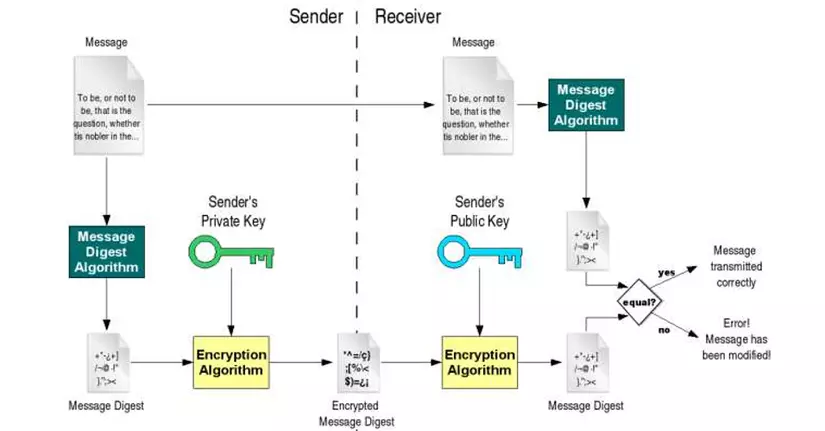
\includegraphics[width=0.8\textwidth]{assets/digital_signature.png} 
    \caption{Quy trình tạo và xác thực chữ ký số sử dụng cặp khóa công khai và bí mật.}
    \label{fig:digital-signature-process}
\end{figure}

Sử dụng khóa bí mật (Private Key) để ký số lên hàm băm (Message Digest) tạo ra một bằng chứng không thể phủ nhận về nguồn gốc của thông điệp. Khi người nhận dùng khóa công khai tương ứng để xác thực thành công, họ biết chắc rằng thông điệp thực sự đến từ chủ sở hữu khóa và không bị chỉnh sửa trên đường truyền. Đây chính là một trong những mục tiêu hoạt động then chốt mà PKI hướng tới nhằm tạo ra sự tin cậy tổng thể.


% ----------------------------------------------------------
\section{Các thành phần PKI}
\label{sec:3.3}

\subsubsection*{CA -- Certificate Authority}
% Ý chính: phát hành + thu hồi chứng chỉ; lưu giữ CRL
% Phân tầng: Root CA (offline, air-gapped) → Intermediate CA → Leaf/End-entity
% Quy trình: CSR → xác minh danh tính → ký cert → publish
Certificate Authority (Tổ chức phát hành chứng chỉ) là trái tim của hệ thống PKI. CA chịu trách nhiệm chính trong việc phát hành, thu hồi chứng chỉ và duy trì danh sách chứng chỉ bị thu hồi (CRL). Để tối ưu hóa tính bảo mật, các CA thường được tổ chức theo cấu trúc phân tầng. Trên cùng là Root CA, nắm giữ khóa quan trọng nhất và thường được giữ ở trạng thái ngoại tuyến (offline, air-gapped) để tránh bị tấn công mạng. Root CA ký cấp phát chứng chỉ cho các Intermediate CA (CA trung gian), và các Intermediate CA này mới là đơn vị trực tiếp tương tác và cấp phát chứng chỉ cho thực thể cuối (Leaf/End-entity). Quy trình cơ bản bao gồm: người dùng tạo Yêu cầu ký chứng chỉ (CSR) $\rightarrow$ CA xác minh danh tính $\rightarrow$ CA dùng khóa bí mật để ký chứng chỉ $\rightarrow$ Công bố chứng chỉ.

\subsubsection*{RA -- Registration Authority}
% Ý chính: tách xác minh danh tính (RA) khỏi ký cert (CA)
% Giảm rủi ro, phân quyền trách nhiệm; ví dụ: RA xác minh hộ chiếu trước khi CA ký
Registration Authority (Tổ chức đăng ký) hoạt động như một cơ quan tiền phương cho CA. Việc tách bạch quá trình xác minh danh tính (thực hiện bởi RA) khỏi quá trình ký chứng chỉ (thực hiện bởi CA) giúp phân quyền trách nhiệm và giảm thiểu rủi ro bảo mật cho hệ thống ký. RA đóng vai trò kiểm tra tính hợp lệ của người nộp đơn. Ví dụ trong thực tế, RA có thể yêu cầu người dùng xuất trình Căn cước công dân hoặc Hộ chiếu để đối chiếu; sau khi RA xác nhận hợp lệ, yêu cầu mới được chuyển tiếp để CA thực hiện thao tác ký số sinh ra chứng chỉ.

\subsubsection*{Repository -- Kho lưu trữ chứng chỉ}
% Ý chính: LDAP directory, HTTP server — nơi client truy vấn cert và CRL public
Kho lưu trữ (Repository) là cơ sở dữ liệu công khai lưu trữ các chứng chỉ đang có hiệu lực và danh sách các chứng chỉ đã bị thu hồi. Kho này thường được triển khai trên các máy chủ thư mục LDAP (Lightweight Directory Access Protocol) hoặc máy chủ HTTP/HTTPS, đảm bảo các client có thể truy vấn nhanh chóng để lấy chứng chỉ của người cần giao tiếp hoặc kiểm tra trạng thái CRL bất cứ lúc nào.

\subsubsection*{CRL -- Certificate Revocation List}
% Ý chính: danh sách cert đã bị thu hồi trước hạn; reason codes (keyCompromise, cACompromise)
% Hạn chế: CRL có thể rất lớn và stale hàng giờ -- giải pháp: delta CRL \cite{RFC5280}
Danh sách chứng chỉ bị thu hồi (CRL) là một tài liệu được CA ký số và phát hành định kỳ, liệt kê số seri của các chứng chỉ đã bị mất hiệu lực trước khi hết hạn. Các lý do thu hồi (reason codes) thường được đi kèm, ví dụ như lộ khóa bí mật (\texttt{keyCompromise}) hoặc bản thân CA bị xâm phạm (\texttt{cACompromise}). Hạn chế lớn của CRL là kích thước tệp có thể phình to rất nhanh và thông tin không được cập nhật tức thời (có thể lỗi thời - stale trong nhiều giờ hoặc vài ngày trước khi bản mới được tải về). Để giảm tải mạng, giải pháp \texttt{delta CRL} \cite{RFC5280} được sử dụng để chỉ tải xuống những thay đổi so với bản CRL đầy đủ trước đó.

\subsubsection*{OCSP -- Online Certificate Status Protocol}
% Ý chính: kiểm tra realtime trạng thái từng cert theo serial number \cite{RFC6960}
% OCSP Stapling \cite{RFC6066}: server pre-fetch response, giải quyết privacy và giảm latency
% Bảng~\ref{tab:revocation}: so sánh CRL vs OCSP vs OCSP Stapling
Giao thức kiểm tra trạng thái chứng chỉ trực tuyến (OCSP) \cite{RFC6960} ra đời nhằm khắc phục độ trễ của CRL. Thay vì tải toàn bộ danh sách, client gửi truy vấn chứa số seri của chứng chỉ đến máy chủ OCSP Responder và nhận về phản hồi theo thời gian thực (Realtime) về trạng thái hợp lệ của chứng chỉ đó. Để giải quyết vấn đề về quyền riêng tư (vì CA biết client đang truy cập trang web nào) và độ trễ (latency) khi client phải tự liên hệ CA, kỹ thuật \textbf{OCSP Stapling} \cite{RFC6066} được áp dụng. Máy chủ web sẽ tự động lấy (pre-fetch) phản hồi OCSP có chữ ký của CA theo định kỳ, sau đó "gắn kèm" (staple) bằng chứng này vào quá trình thiết lập kết nối TLS ban đầu với client.

\begin{table}[h]
    \centering
    \caption{So sánh các phương pháp kiểm tra trạng thái thu hồi chứng chỉ}
    \label{tab:revocation}
    \begin{tabular}{|p{3cm}|p{4cm}|p{4cm}|p{4cm}|}
        \hline
        \textbf{Tiêu chí} & \textbf{CRL} & \textbf{OCSP} & \textbf{OCSP Stapling} \\
        \hline
        Độ trễ cập nhật & Cao (phụ thuộc chu kỳ tải) & Thấp (thời gian thực) & Thấp (thời gian thực, có cache) \\
        \hline
        Chi phí băng thông & Rất cao (tải toàn bộ list) & Thấp & Rất thấp \\
        \hline
        Quyền riêng tư & Tốt (Client kiểm tra cục bộ) & Kém (CA biết lịch sử duyệt web) & Tốt (Client không gọi trực tiếp CA) \\
        \hline
    \end{tabular}
\end{table}


% ----------------------------------------------------------
\section{Chu kỳ sống của chứng chỉ}
\label{sec:3.4}
% Ý chính: Tạo keypair → CSR → xác minh danh tính → phát hành → sử dụng → gia hạn / thu hồi
% Certificate lifecycle automation (ACME, SCEP, EST) ngày càng quan trọng
% Hình~\ref{fig:cert-lifecycle}: sơ đồ lifecycle
Hoạt động của PKI phụ thuộc vào việc quản lý chặt chẽ vòng đời (lifecycle) của một chứng chỉ số. Chu kỳ sống này bao gồm các giai đoạn tuần tự:
\begin{enumerate}
    \item \textbf{Tạo cặp khóa (Keypair Generation):} Thực thể tự tạo Khóa công khai và Khóa bí mật một cách an toàn.
    \item \textbf{Tạo yêu cầu (CSR Creation):} Gói Khóa công khai và các thông tin định danh vào một bản tin CSR (Certificate Signing Request).
    \item \textbf{Xác minh (Verification):} RA/CA kiểm tra tính hợp lệ của thông tin và quyền sở hữu tên miền/tổ chức.
    \item \textbf{Phát hành (Issuance):} CA ký điện tử lên CSR để tạo ra chứng chỉ số hợp lệ.
    \item \textbf{Sử dụng (Usage):} Chứng chỉ được triển khai trên hệ thống (web server, email) để thực hiện mã hóa và xác thực.
    \item \textbf{Gia hạn / Thu hồi (Renewal / Revocation):} Trước khi hết hạn, chứng chỉ cần được gia hạn. Nếu khóa bí mật bị lộ hoặc thông tin không còn đúng, chứng chỉ sẽ bị đưa vào quá trình thu hồi (đưa vào CRL hoặc báo trạng thái qua OCSP).
\end{enumerate}

Với sự bùng nổ của quy mô dịch vụ đám mây và microservices, việc cấu hình thủ công không còn khả thi. Tự động hóa vòng đời chứng chỉ (Certificate Lifecycle Automation) thông qua các giao thức như ACME (được Let's Encrypt sử dụng phổ biến), SCEP, hoặc EST ngày càng đóng vai trò quan trọng yếu giúp đảm bảo hệ thống không bị gián đoạn dịch vụ do chứng chỉ hết hạn.

\begin{figure}[h]
    \centering
    % Placeholder cho hình ảnh kiến trúc / chu kỳ sống. Bạn có thể chèn file hình vào cấu trúc thư mục LaTeX của mình.
    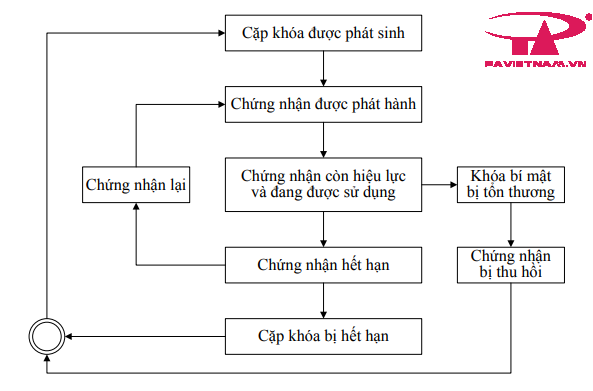
\includegraphics[width=0.6\textwidth]{assets/cert_lifecycle.png}
    \caption{Sơ đồ chu kỳ sống của chứng chỉ số trong hệ thống PKI}
    \label{fig:cert-lifecycle}
\end{figure}
